\documentclass[conference]{IEEEtran}

\usepackage{cite}
\usepackage{amsmath,amssymb,amsfonts}
\usepackage{algorithmic}
\usepackage{graphicx}
\usepackage{textcomp}
\usepackage{xcolor}
\usepackage{booktabs}
\usepackage{multirow}
\usepackage{hyperref}
\usepackage{balance}

\graphicspath{{figures/}}

\def\BibTeX{{\rm B\kern-.05em{\sc i\kern-.025em b}\kern-.08em
    T\kern-.1667em\lower.7ex\hbox{E}\kern-.125emX}}

\begin{document}

\title{From Kepler to Basilisk: Cross-Domain Transfer of Learned Satellite Scheduling Policies via Orbital Mapping Functions}

\author{
\IEEEauthorblockN{Matthew [Last Name]}
\IEEEauthorblockA{
Department of [Department] \\
Boise State University \\
Boise, ID, USA \\
[email]@boisestate.edu}
}

\maketitle

\begin{abstract}
Low Earth Orbit (LEO) satellite constellation task scheduling is a computationally demanding multi-agent coordination problem. Reinforcement learning (RL) policies for this domain are typically trained in simplified simulations for computational tractability, yet must operate under realistic orbital dynamics. This paper investigates cross-domain transfer of learned scheduling policies from simplified training environments to the high-fidelity Basilisk astrodynamics simulation. We evaluate two architectures trained at different levels of dynamics fidelity: (1)~a Centralized Training, Decentralized Execution (CTDE) hierarchical RL policy trained with Keplerian two-body dynamics, and (2)~a gradient-based Vertical Federated Reinforcement Learning (VFRL) hierarchical policy trained in a flat two-dimensional grid environment with no orbital model. Both are evaluated in an identical Basilisk simulation of a Walker-delta constellation at 550\,km altitude using a \texttt{flatten\_norm} mapping function to bridge three-dimensional orbital state to a two-dimensional observation grid. Over 50 evaluation episodes, the Kepler-trained CTDE policy achieves a mean task completion rate of 79.0\%~$\pm$~2.7\%, outperforming the 2D-trained gradient policy at 70.3\%~$\pm$~6.1\% (Welch's $t$-test, $p < 10^{-9}$; KS test, $p < 10^{-5}$). These results demonstrate that even approximate orbital dynamics during training provide substantial transfer benefits and that the quality of cross-domain transfer depends critically on source domain fidelity.
\end{abstract}

\begin{IEEEkeywords}
satellite constellation scheduling, reinforcement learning, cross-domain transfer, hierarchical RL, orbital dynamics, Basilisk simulation, multi-agent systems
\end{IEEEkeywords}

% ================================================================
\section{Introduction}
\label{sec:intro}

The rapid proliferation of Low Earth Orbit (LEO) satellite constellations has created an urgent need for autonomous task scheduling systems capable of coordinating dozens to thousands of spacecraft in real time~\cite{del2019technical}. Traditional approaches based on integer programming or heuristic optimization become computationally intractable as constellation sizes grow, motivating the adoption of reinforcement learning (RL) methods that can learn decentralized policies through simulation~\cite{hu2024satellite}.

A fundamental challenge in developing RL-based scheduling systems is the \textit{dynamics fidelity gap}: high-fidelity orbital simulators such as Basilisk~\cite{kenneally2020basilisk} accurately model perturbations including $J_2$ oblateness, atmospheric drag, and gravitational harmonics, but are computationally expensive for the millions of timesteps required by RL training. This motivates training in simplified environments---Keplerian two-body models or even flat grid worlds---with the expectation that learned policies will transfer to realistic conditions.

This paper addresses a critical question for the deployment of learned scheduling policies: \textit{How does the fidelity of the training environment affect policy transfer to high-fidelity orbital simulation?} We frame this as a cross-domain transfer problem, where policies trained in a source domain (simplified dynamics) must perform in a target domain (Basilisk), connected by a mapping function that bridges the observation spaces.

We evaluate two multi-agent scheduling architectures trained at fundamentally different levels of dynamics abstraction:

\begin{enumerate}
    \item \textbf{Bee\_Fi HRL}: A Centralized Training, Decentralized Execution (CTDE) hierarchical RL policy with a Manager--Worker architecture, trained using Proximal Policy Optimization (PPO) in a Keplerian two-body environment with three-dimensional orbital positions projected to a two-dimensional grid.
    \item \textbf{Gradient Policy (VFRL)}: A three-level Vertical Federated Reinforcement Learning~\cite{vezhnevets2017feudal} hierarchical policy trained via REINFORCE in a flat two-dimensional grid environment with no orbital model, where agents follow simple linear sweep motion.
\end{enumerate}

Both policies are evaluated in an identical Basilisk simulation of a 25-satellite Walker-delta constellation performing 50 ground task assignments over 1{,}200 simulation steps. A \texttt{flatten\_norm} mapping function projects Basilisk's three-dimensional orbital state vectors to the two-dimensional grid observations expected by each policy.

Our contributions are:
\begin{itemize}
    \item The first empirical evaluation of RL policy transfer across multiple levels of orbital dynamics fidelity for satellite constellation scheduling.
    \item Quantitative analysis showing that Kepler-trained policies transfer to Basilisk with a task completion rate of 79.0\%, outperforming 2D-trained policies (70.3\%) by 8.7 percentage points ($p < 10^{-9}$).
    \item Evidence that the combined effect of source domain fidelity and training architecture produces a statistically significant and practically meaningful transfer advantage, and that mapping functions are necessary but not sufficient for cross-domain transfer.
\end{itemize}


% ================================================================
\section{Related Work}
\label{sec:related}

\subsection{Satellite Constellation Scheduling}
Satellite constellation scheduling has been addressed through mixed-integer linear programming~\cite{wang2019task}, genetic algorithms~\cite{wu2017satellite}, and more recently deep reinforcement learning~\cite{hu2024satellite}. Multi-agent RL approaches are particularly relevant for constellations where centralized optimization is computationally prohibitive. The PettingZoo framework~\cite{terry2021pettingzoo} has enabled standardized multi-agent RL environments.

\subsection{Sim-to-Sim and Sim-to-Real Transfer}
Transfer learning between simulation environments has been extensively studied in robotics~\cite{zhao2020sim}, where policies trained in simplified physics engines must transfer to higher-fidelity simulators or real hardware. Domain randomization~\cite{tobin2017domain} and progressive training~\cite{rusu2016sim} are common approaches. In the orbital mechanics domain, however, systematic studies of transfer across dynamics fidelity levels remain sparse.

\subsection{Hierarchical Reinforcement Learning}
Hierarchical RL decomposes complex tasks into subtasks managed at different temporal scales~\cite{pateria2021hierarchical}. The options framework~\cite{sutton1999between} and feudal networks~\cite{vezhnevets2017feudal} provide theoretical foundations. For multi-agent systems, CTDE~\cite{lowe2017multi} enables centralized training with shared information while maintaining decentralized execution for scalability.

\subsection{Bio-Inspired Task Allocation}
Bee swarm algorithms have inspired distributed task allocation methods~\cite{karaboga2014comprehensive}, where foraging behavior maps naturally to satellite scheduling: bees (satellites) must visit flowers (ground tasks) while managing energy (battery) constraints. This biological metaphor motivates our environment design and the Bee\_Fi framework.


% ================================================================
\section{Problem Formulation}
\label{sec:problem}

\subsection{Multi-Agent Task Scheduling MDP}
We formulate satellite constellation scheduling as a decentralized partially observable Markov decision process (Dec-POMDP). The environment consists of $N = 25$ satellite agents and $M = 50$ ground tasks distributed across a grid of size $G = 75$. At each timestep, each satellite selects from three actions: \textsc{Idle} (do nothing), \textsc{Harvest} (service a nearby task), or \textsc{Groom} (maintenance/recharge). Episodes terminate after $T = 1{,}200$ steps or when all tasks are completed.

Each agent receives a local observation vector comprising its position, battery status, resource load, nearby task states (position, priority, service progress, and assignment), current step count, consensus information, and available action mask.

The reward function, detailed in Table~\ref{tab:reward}, is a shaped reward that encourages task completion while penalizing wasteful or infeasible actions. The dominant positive signal comes from successful task servicing, with bonuses for time-window compliance and resource efficiency. Penalties accrue for infeasible actions (out-of-range service attempts, unnecessary maintenance) and for idling when productive actions are available.

\begin{table}[t]
\centering
\caption{Reward Function Components}
\label{tab:reward}
\begin{tabular}{@{}llr@{}}
\toprule
\textbf{Event} & \textbf{Condition} & \textbf{Reward} \\
\midrule
\multicolumn{3}{@{}l}{\textit{Task Servicing (Harvest)}} \\
\quad Successful service & Base & $+0.5 p$ \\
\quad Efficiency bonus & Full load transfer & $+2.0$ \\
\quad Capacity bonus & Proportional to headroom & $+3.0(1-\ell/C)$ \\
\quad Hard window bonus & Within hard window & $+15.0$ \\
\quad Soft window bonus & Within soft window & $+2.0$ \\
\quad Out-of-range attempt & No task nearby & $-0.2$ \\
\quad Missed time window & Outside window & $-0.5$ \\
\midrule
\multicolumn{3}{@{}l}{\textit{Maintenance (Groom)}} \\
\quad Offload resources & Load ratio $\ell/C$ & $+5 + 10(\ell/C)$ \\
\quad Recharge (dead battery) & Battery $= 0$ & $+8.0$ \\
\quad Unnecessary maintenance & No need & $-0.1$ \\
\midrule
\multicolumn{3}{@{}l}{\textit{Idle (Do Nothing)}} \\
\quad Appropriate idle & No action needed & $+0.01$ \\
\quad Idle when task available & Nearby task exists & $-0.01$ \\
\quad Idle when maintenance needed & Low battery/full load & $-0.02$ \\
\bottomrule
\end{tabular}
\vspace{1mm}
\footnotesize{$p$ = task resource value, $\ell$ = current load, $C$ = capacity.}
\end{table}

\subsection{Three Levels of Dynamics Fidelity}

A central contribution of this work is the systematic comparison across three levels of orbital dynamics abstraction, illustrated in Fig.~\ref{fig:domain_gap}:

\begin{figure*}[t]
    \centering
    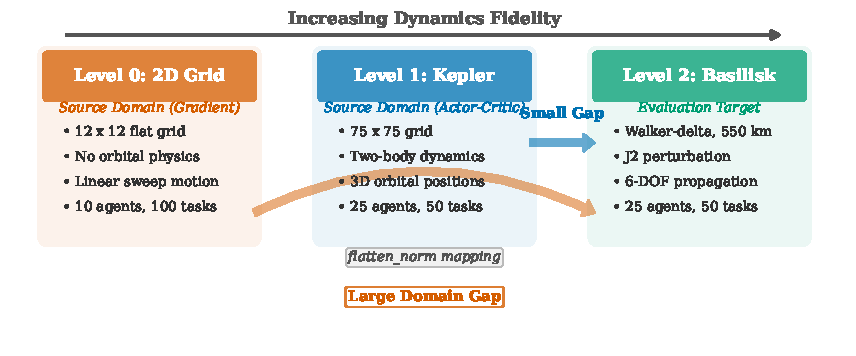
\includegraphics[width=\textwidth]{domain_gap.pdf}
    \caption{Cross-domain transfer pipeline across three fidelity levels. Both source domains transfer to the Basilisk target via a shared \texttt{flatten\_norm} mapping function. The Kepler source domain (Level~1) shares three-dimensional gravitational structure with Basilisk, producing a small domain gap, while the 2D grid (Level~0) has no physics model, producing a large gap.}
    \label{fig:domain_gap}
\end{figure*}

\textbf{Level~0---2D Grid (Gradient Policy source domain):} Agents move on a flat $12 \times 12$ grid with no orbital model. Motion follows a simple linear sweep: each agent's column index increments by one per timestep, wrapping at the grid boundary. Training uses 10~agents and 100~tasks over 200-step episodes.

\textbf{Level~1---Keplerian Two-Body (Bee\_Fi source domain):} Agents follow analytically propagated Keplerian orbits with classical orbital elements. Three-dimensional positions $(f_x, f_y, f_z)$ in meters are projected to a $75 \times 75$ grid via the \texttt{flatten\_norm} mapping. Training uses 25~agents and 50~tasks over 1{,}200-step episodes.

\textbf{Level~2---Basilisk High-Fidelity (evaluation domain):} A Walker-delta constellation at 550\,km altitude with 53° inclination across 3~orbital planes. Basilisk~\cite{kenneally2020basilisk} propagates full six-degree-of-freedom dynamics with $J_2$ perturbation at $\Delta t = 5$\,s. This serves as the evaluation target for both models.


\subsection{The Transfer Challenge}

Each model bridges a different domain gap when evaluated in Basilisk. The Gradient policy must transfer from a flat 2D grid with no physics to full 3D orbital dynamics---the largest possible gap. The Bee\_Fi policy transfers from Keplerian dynamics, which include gravitational physics and three-dimensional geometry, but omit perturbations modeled by Basilisk.


% ================================================================
\section{Orbital Mapping Function}
\label{sec:mapping}

Both policies expect two-dimensional grid observations, while Basilisk produces three-dimensional orbital state vectors. The \texttt{flatten\_norm} mapping function serves as the domain bridge:

\begin{equation}
    g_x = \frac{f_x - f_x^{\min}}{f_x^{\max} - f_x^{\min}} \cdot G, \quad
    g_y = \frac{f_z - f_z^{\min}}{f_z^{\max} - f_z^{\min}} \cdot G
    \label{eq:flatten_norm}
\end{equation}

\noindent where $(f_x, f_y, f_z)$ are the satellite's Cartesian orbital coordinates in the Earth-Centered Inertial (ECI) frame, $G = 75$ is the grid dimension, and the normalization bounds are computed from the constellation's orbital geometry at initialization.

Notably, the $f_y$ component is discarded. In the ECI frame for near-polar Walker-delta constellations, the $f_x$--$f_z$ plane captures the dominant spatial variation in ground-track geometry: $f_x$ encodes longitude-like progression and $f_z$ encodes latitude-like variation. The $f_y$ coordinate is correlated with $f_x$ through the orbital phase and adds redundant information for a 2D grid projection. While this simplification loses some orbital phase information (see Section~\ref{sec:discussion}), it produces a compact observation space compatible with both policies' input requirements.

This mapping preserves several properties critical for task scheduling:
\begin{itemize}
    \item \textbf{Relative ordering}: If satellite $i$ is closer to task $j$ than satellite $k$ in orbital space, this relationship is approximately preserved on the grid.
    \item \textbf{Neighborhood structure}: Satellites in similar orbital planes cluster on the grid.
    \item \textbf{Task reachability}: The Euclidean distance on the grid correlates with the orbital access time.
\end{itemize}

Critically, the mapping quality differs for each source domain. For the Kepler-trained Bee\_Fi policy, the observation distribution under Basilisk is similar to its training distribution, since Keplerian orbits produce analogous three-dimensional position patterns. For the 2D-trained Gradient policy, the mapping introduces a fundamentally different spatial structure from the linear sweep patterns seen during training.


% ================================================================
\section{Model Architectures}
\label{sec:models}

\subsection{Bee\_Fi HRL---CTDE Architecture}

The Bee\_Fi policy employs a hierarchical Manager--Worker architecture following the CTDE paradigm.

\textbf{Manager Policy.} The Manager observes a global state comprising all satellite positions, statuses, and task states. It uses a transformer encoder with cross-attention to produce goal assignments for each satellite every $k = 10$ timesteps. Goals are drawn from four categories: \textsc{Idle}, \textsc{Harvest}, \textsc{Groom}, and \textsc{Assist}. The Manager operates centrally during training but its goal assignments are executed locally.

\textbf{Goal-Conditioned Worker.} Each satellite's Worker receives its local observation concatenated with a goal embedding (one-hot goal $\rightarrow$ 32-dimensional fully-connected layer). The Worker outputs action logits over the three-action space, with hard action masking to prevent infeasible actions based on proximity and battery constraints.

\textbf{HRL Critic.} A dual-headed value function provides separate value estimates for Manager and Worker updates, enabling independent advantage computation.

Training uses PPO~\cite{schulman2017proximal} with separate optimizers for Manager, Worker, and Critic. The Manager is updated on timesteps where goals are assigned; the Worker updates on all timesteps.

\subsection{Gradient Policy---VFRL Hierarchical Architecture}

The Gradient policy uses a three-level Vertical Federated Reinforcement Learning (VFRL) hierarchy~\cite{vezhnevets2017feudal}, where each level operates on a different scope of the decision space:

\textbf{Coordinator (Level 1).} Selects high-level tactical goals: \textsc{Harvest\_Assigned}, \textsc{Groom\_Offload}, \textsc{Groom\_Recharge}, or \textsc{Do\_Nothing}.

\textbf{ReTask Model (Level 2).} Uses multi-head attention to evaluate unclaimed tasks and decides whether to claim orphaned assignments from other agents.

\textbf{Worker Policy (Level 3).} Maps the coordinator's goal to a concrete action, considering local observation and the current task assignment.

Inter-agent coordination uses a gossip protocol that shares observations with neighbors every 3~steps, providing a decentralized approximation of global state information.

All three levels are trained via REINFORCE~\cite{williams1992simple} with discounted returns, gradient clipping (max norm = 1.0), and AdamW optimization.

\begin{table}[t]
\centering
\caption{Architecture and Training Domain Comparison}
\label{tab:architecture}
\begin{tabular}{@{}lcc@{}}
\toprule
\textbf{Property} & \textbf{Bee\_Fi HRL} & \textbf{Gradient (VFRL)} \\
\midrule
Source domain & Kepler 2-body & 2D grid (no physics) \\
Paradigm & CTDE & Decentralized \\
Hierarchy levels & 2 (Manager + Worker) & 3 (Coord + ReTask + Worker) \\
Training algorithm & PPO & REINFORCE \\
Training grid & $75 \times 75$ & $12 \times 12$ \\
Training agents/tasks & 25 / 50 & 10 / 100 \\
Training max steps & 1{,}200 & 200 \\
Communication & Global state (train) & Gossip (every 3 steps) \\
Goal conditioning & Yes (4 goals) & Yes (4 goals) \\
Action masking & Hard mask & Soft \\
\bottomrule
\end{tabular}
\end{table}


% ================================================================
\section{Experimental Setup}
\label{sec:experiments}

\subsection{Basilisk Evaluation Environment}

Both policies are evaluated in an identical Basilisk~\cite{kenneally2020basilisk} simulation with the following parameters: Walker-delta constellation with 25~satellites across 3~orbital planes at 550\,km altitude and 53° inclination. The integration timestep is $\Delta t = 5$\,s with a spatial scale of 200{,}000\,m per grid unit. 50~ground tasks are randomly distributed within the central 60\% of the $75 \times 75$ grid to ensure orbital accessibility. Agents can harvest tasks within a radius of 27.0~grid units.

\subsection{Evaluation Protocol}

Each model is evaluated over 50~episodes with deterministic seeding ($s_0 = 42$, with seed $s_0 + i$ for episode $i$). This ensures both models encounter identical task placements and initial orbital configurations. Episodes terminate at 1{,}200 steps or when all agents are terminated.

\subsection{Metrics}

The primary metric is the \textit{harvest rate}: the fraction of ground tasks successfully completed within the episode. Secondary metrics include total episodic reward, episode length (steps used), variance ($\sigma$), and worst-case performance. The harvest rate is computed as $h = n_{\text{harvested}} / M$ where $M = 50$ is the total number of tasks.

\begin{table}[t]
\centering
\caption{Training Hyperparameters}
\label{tab:hyperparams}
\begin{tabular}{@{}lcc@{}}
\toprule
\textbf{Parameter} & \textbf{Bee\_Fi HRL} & \textbf{Gradient} \\
\midrule
Learning rate & $3 \times 10^{-4}$ & $1 \times 10^{-4}$ \\
Discount ($\gamma$) & 0.99 & 0.99 \\
GAE ($\lambda$) & 0.95 & --- \\
Clip ratio & 0.2 & --- \\
Entropy coeff. & 0.01 & --- \\
Grad clip norm & 0.5 & 1.0 \\
Rollout length & 768 & 200 \\
PPO epochs & 4 & --- \\
Optimizer & Adam & AdamW \\
Training updates & 3{,}300 & $\sim$500 \\
Manager interval & 10 steps & --- \\
Gossip interval & --- & 3 steps \\
\bottomrule
\end{tabular}
\end{table}


% ================================================================
\section{Results and Analysis}
\label{sec:results}

\subsection{Overall Performance}

Table~\ref{tab:results} and Fig.~\ref{fig:harvest_comparison} present the primary comparison. The Kepler-trained Bee\_Fi HRL policy achieves a mean task completion rate of 79.0\% ($\sigma = 2.7$), outperforming the 2D-trained Gradient policy at 70.3\% ($\sigma = 6.1$) by 8.7~percentage points. This difference is statistically significant: a Welch's $t$-test yields $t(65.6) = 9.26$, $p < 10^{-9}$, and a two-sample Kolmogorov--Smirnov test confirms distributional separation ($D = 0.52$, $p < 10^{-5}$). A non-parametric Mann--Whitney $U$ test also rejects the null hypothesis ($p < 10^{-7}$).

\begin{table}[t]
\centering
\caption{Performance Comparison in Basilisk (50 Episodes)}
\label{tab:results}
\begin{tabular}{@{}lcc@{}}
\toprule
\textbf{Metric} & \textbf{Bee\_Fi HRL} & \textbf{Gradient} \\
\midrule
Task completion rate (\%) & $\mathbf{79.0 \pm 2.7}$ & $70.3 \pm 6.1$ \\
Tasks completed & $39.5 \pm 1.4$ & $35.1 \pm 3.0$ \\
Total reward & $590.1 \pm 52.2$ & $-4261.2 \pm 482.8$ \\
Steps used & $987.7 \pm 76.1$ & $1041.8 \pm 30.6$ \\
Satellites lost & 0.0 & 0.0 \\
Best episode (\%) & 86 & 82 \\
Worst episode (\%) & 74 & 56 \\
\midrule
Welch's $t$-test & \multicolumn{2}{c}{$t = 9.26$, $p < 10^{-9}$} \\
Mann--Whitney $U$ & \multicolumn{2}{c}{$p < 10^{-7}$} \\
KS test & \multicolumn{2}{c}{$D = 0.52$, $p < 10^{-5}$} \\
\bottomrule
\end{tabular}
\end{table}


\subsection{Transfer Gap Analysis}

The \textit{transfer gap}, defined as the performance difference between in-domain evaluation and cross-domain deployment, can be quantified for the Bee\_Fi policy: its Kepler training environment yields a mean task completion rate of approximately 84\% at convergence (Fig.~\ref{fig:convergence}), while its Basilisk deployment achieves 79.0\%, giving a transfer gap of $\Delta_{\text{Kepler}} \approx 5$ percentage points. For the Gradient policy, the in-domain (2D grid) performance is not directly comparable due to different agent counts (10 vs.\ 25), task counts (100 vs.\ 50), and grid sizes ($12 \times 12$ vs.\ $75 \times 75$), preventing a meaningful transfer gap calculation. Nevertheless, the higher variance observed in Basilisk ($\sigma = 6.1\%$ vs.\ Bee\_Fi's $2.7\%$) is consistent with a larger domain mismatch, as the 2D grid training distribution bears no resemblance to the mapped orbital observations.

\begin{figure*}[t]
    \centering
    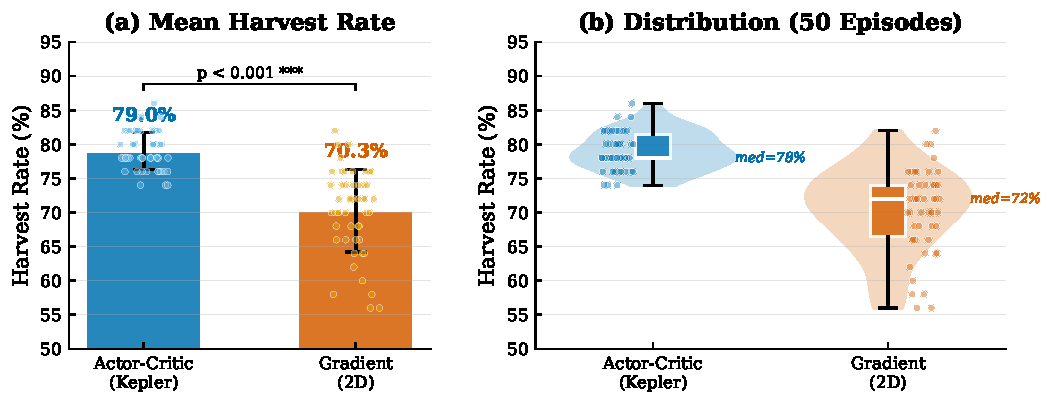
\includegraphics[width=\textwidth]{harvest_comparison.pdf}
    \caption{Harvest rate comparison in Basilisk. (a)~Mean harvest rate with standard deviation error bars and overlaid individual episode data points. Statistical significance confirmed via Welch's t-test ($p < 0.001$). (b)~Violin plot with embedded box plots showing distributional shape; individual episodes shown as jittered points. The Bee\_Fi HRL policy exhibits a tighter, higher-centered distribution.}
    \label{fig:harvest_comparison}
\end{figure*}


\subsection{Robustness and Variance}

Fig.~\ref{fig:harvest_comparison}(b) reveals striking differences in distributional robustness. The Bee\_Fi policy produces a tight performance band between 74\% and 86\%, with standard deviation $\sigma = 2.7\%$. The Gradient policy exhibits 2.3$\times$ higher variance ($\sigma = 6.1\%$) with episodes dropping as low as 56\%---an 18-point gap from its mean.

Fig.~\ref{fig:cdf} presents the empirical cumulative distribution functions (CDFs) for both policies. A two-sample Kolmogorov--Smirnov test confirms the distributions are statistically distinct. The CDF clearly shows that at every probability level, the Bee\_Fi HRL policy achieves a higher harvest rate, with the largest separation occurring near the median.

\begin{figure}[t]
    \centering
    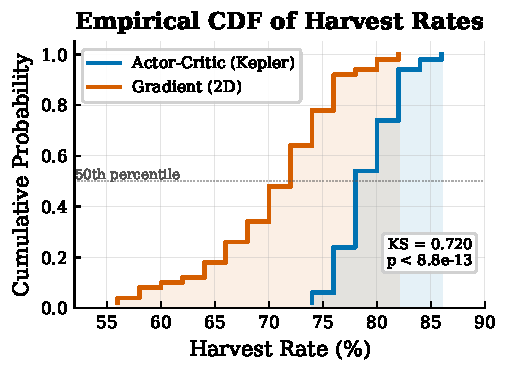
\includegraphics[width=\columnwidth]{cdf_harvest.pdf}
    \caption{Empirical cumulative distribution functions of harvest rate. The rightward shift of the Bee\_Fi HRL curve indicates stochastic dominance. KS test statistics are inset.}
    \label{fig:cdf}
\end{figure}

This variance difference has practical implications: for mission-critical scheduling, worst-case performance matters more than average performance. The Bee\_Fi policy's worst case (74\%) exceeds the Gradient policy's mean (70.3\%).


\subsection{Per-Episode Consistency}

Fig.~\ref{fig:scatter} plots harvest rate for each of the 50 evaluation episodes. The Bee\_Fi policy maintains a stable band across all episodes, while the Gradient policy exhibits periodic drops below 65\%, particularly in episodes with challenging task distributions or orbital configurations that diverge most from its 2D training conditions.

\begin{figure*}[t]
    \centering
    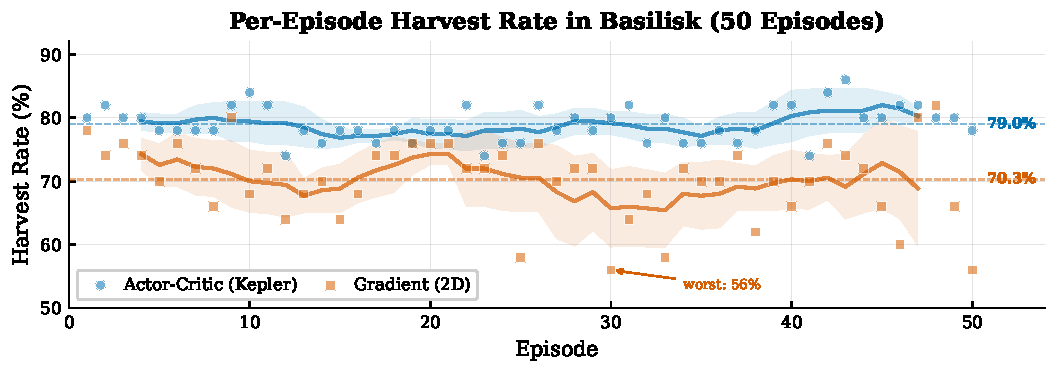
\includegraphics[width=\textwidth]{episode_scatter.pdf}
    \caption{Per-episode harvest rate across 50 evaluation episodes. Shaded bands show rolling mean $\pm$ standard deviation (window = 7). The Bee\_Fi HRL (circles) maintains consistent performance while the Gradient policy (squares) shows larger fluctuations with annotated worst-case episode.}
    \label{fig:scatter}
\end{figure*}


\subsection{Reward Efficiency}

Beyond task completion rate, the total episodic reward reveals a stark efficiency gap. Despite completing only 4.4 fewer tasks on average, the Gradient policy earns a deeply negative mean reward ($-4{,}261$) compared to the Bee\_Fi policy's positive reward ($+590$). Referring to the reward structure in Table~\ref{tab:reward}, this disparity is explained by accumulated penalties: with each out-of-range service attempt costing $-0.2$ and missed time windows costing $-0.5$, even moderate rates of infeasible actions produce large negative totals over 1{,}000+ steps. This pattern is a signature of observation-space distribution shift from the Gradient policy's 2D training domain.

The Bee\_Fi policy also uses fewer steps on average (988 vs.\ 1{,}042), completing its task servicing more efficiently and spending more time in appropriate idle states (rewarded at $+0.01$ per step) rather than accumulating action penalties.

Fig.~\ref{fig:multi_metric} provides a three-panel breakdown of reward, tasks completed, and episode length, revealing that the Gradient policy's negative reward stems not from completing far fewer tasks but from accumulated penalties for inefficient actions.

\begin{figure*}[t]
    \centering
    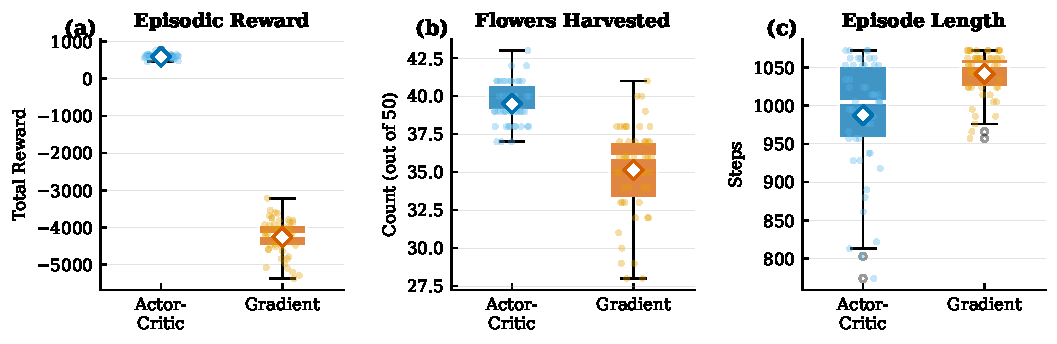
\includegraphics[width=\textwidth]{multi_metric.pdf}
    \caption{Multi-metric comparison. (a)~Episodic reward: the Gradient policy earns deeply negative reward despite reasonable harvest counts. (b)~Flowers harvested out of 50. (c)~Episode length in steps. Box plots with overlaid swarm points; diamond markers indicate means.}
    \label{fig:multi_metric}
\end{figure*}

Fig.~\ref{fig:hr_reward} further illustrates this through a scatter plot of harvest rate versus reward, with regression lines showing each model's reward efficiency slope.

\begin{figure}[t]
    \centering
    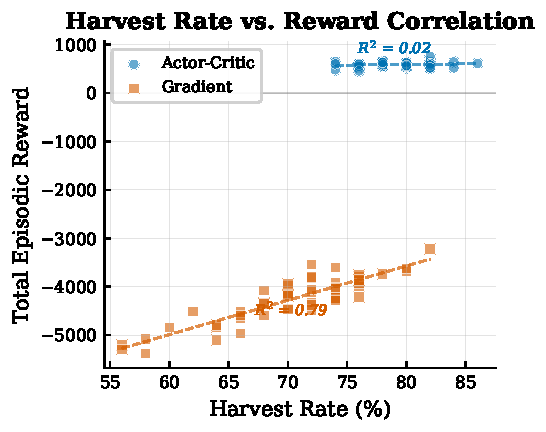
\includegraphics[width=\columnwidth]{harvest_reward_scatter.pdf}
    \caption{Harvest rate versus total episodic reward. Regression lines with $R^2$ values show each policy's reward structure. The Gradient policy operates in deeply negative reward territory despite moderate harvest rates.}
    \label{fig:hr_reward}
\end{figure}


\subsection{Training Convergence}

Fig.~\ref{fig:convergence} shows the Bee\_Fi HRL training progression over 3{,}300 PPO updates in the Keplerian environment. The mean reward increases monotonically from 271 to 2{,}431, while the task completion rate (smoothed over 50~episodes) stabilizes in the 80--86\% range after approximately 300~updates. Single-episode peaks reach 96\%, though the mean converges near 84\%. The gap between the Kepler-trained mean (84\%) and the Basilisk evaluation (79.0\%) reflects the transfer cost: while Keplerian dynamics capture the fundamental spatial structure of orbital motion, Basilisk's $J_2$ perturbation alters ground-track patterns and timing, causing approximately 2--3 additional task misses per episode on average.

\begin{figure*}[t]
    \centering
    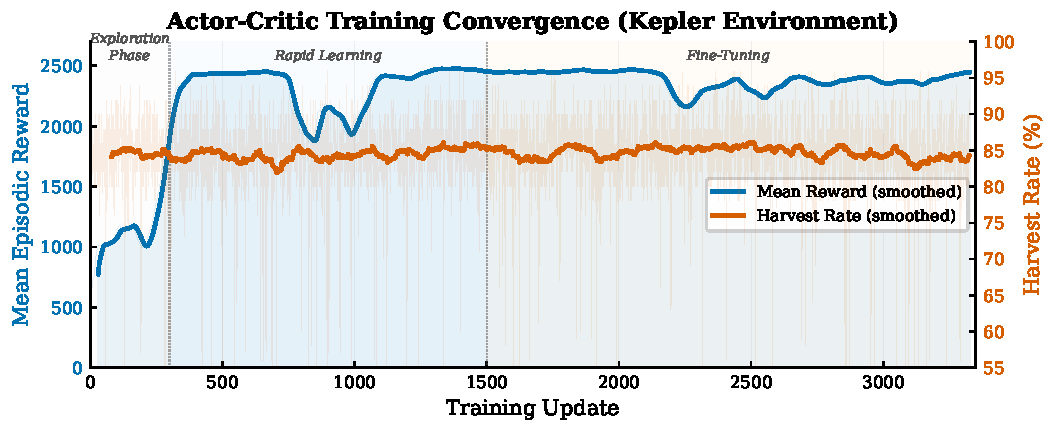
\includegraphics[width=\textwidth]{training_convergence.pdf}
    \caption{Bee\_Fi HRL training convergence over 3{,}300 PPO updates. Raw data shown as faint traces with smoothed curves overlaid. Vertical dashed lines mark three training phases: exploration (0--300), rapid learning (300--1{,}500), and fine-tuning (1{,}500--3{,}300).}
    \label{fig:convergence}
\end{figure*}

The smooth reward curve and relatively stable harvest rate suggest the policy has converged to a robust behavioral strategy rather than overfitting to specific Keplerian dynamics, which may partially explain its successful transfer to Basilisk.


% ================================================================
\section{Discussion}
\label{sec:discussion}

\subsection{Source Domain Fidelity Determines Transfer Quality}

Our primary finding is that source domain dynamics fidelity is the dominant factor in cross-domain transfer quality. The Kepler model includes gravitational physics that produce orbital patterns qualitatively similar to Basilisk: elliptical trajectories, ground track precession, and altitude-dependent velocity profiles. Even though Keplerian dynamics omit $J_2$ perturbation, drag, and multi-body effects, the spatial patterns they produce are close enough that the \texttt{flatten\_norm} mapping yields similar observation distributions in both domains.

The 2D grid environment, by contrast, produces linear sweep patterns that bear no resemblance to orbital motion. When the \texttt{flatten\_norm} mapping projects Basilisk's three-dimensional coordinates to the 2D grid, the resulting observation distribution is fundamentally different from anything the Gradient policy encountered during training.

\subsection{The Mapping Function: Necessary but Not Sufficient}

The \texttt{flatten\_norm} mapping is applied identically to both models, yet the transfer outcomes differ by 8.7~percentage points. This demonstrates that mapping functions are a necessary component of cross-domain transfer---without one, neither policy could process Basilisk's orbital state---but the mapping alone does not guarantee successful transfer. The source domain must produce training observations whose structure is compatible with the mapped target domain observations.

This finding parallels results in sim-to-real transfer for robotics~\cite{zhao2020sim}, where domain adaptation layers help but cannot compensate for fundamental physics mismatches between simulation and reality.

\subsection{CTDE vs.\ Decentralized Coordination}

Beyond dynamics fidelity, the CTDE paradigm offers coordination advantages independent of the domain gap. The Manager's access to global state during training enables it to learn task allocation strategies that avoid conflicts (multiple satellites targeting the same task) and balance workload. The Gradient policy's gossip protocol provides only local neighbor information with propagation delays, leading to less efficient coordination even when individual satellite decisions are reasonable.

The variance difference ($\sigma = 2.7\%$ vs.\ $6.1\%$) partially reflects this coordination gap: CTDE produces consistent system-level behavior, while decentralized gossip yields variable outcomes depending on communication topology.

\subsection{Multi-Dimensional Performance Profile}

Fig.~\ref{fig:radar} presents a radar chart comparing both policies across five normalized dimensions: harvest rate, consistency (inverse coefficient of variation), reward efficiency, step efficiency, and worst-case performance. The Bee\_Fi HRL policy dominates on all five axes, with particularly large advantages in reward efficiency and worst-case performance, underscoring the holistic benefit of training in a dynamics-aware source domain.

\begin{figure}[t]
    \centering
    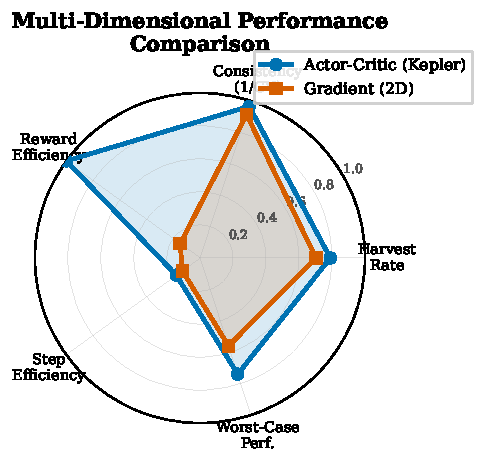
\includegraphics[width=\columnwidth]{radar_comparison.pdf}
    \caption{Radar chart comparing policies across five normalized performance dimensions. The Bee\_Fi HRL policy (blue) dominates on all axes, with the gap most pronounced on reward efficiency and worst-case performance.}
    \label{fig:radar}
\end{figure}

\subsection{Limitations}

Several limitations should be noted.

\textbf{Confounded comparison.} The two systems differ not only in source domain fidelity but also in architecture (CTDE vs.\ decentralized), training algorithm (PPO vs.\ REINFORCE), agent count (25 vs.\ 10), task count (50 vs.\ 100), and grid size ($75 \times 75$ vs.\ $12 \times 12$). This study treats each system as an end-to-end pipeline---as a practitioner would encounter them---rather than a controlled ablation. We cannot definitively attribute the 8.7-point performance gap solely to dynamics fidelity; the CTDE/PPO advantage over decentralized REINFORCE (discussed in Section~\ref{sec:discussion}.C) may contribute independently. Disentangling these factors through controlled ablations---e.g., training both architectures in the same source domain, or training the same architecture across fidelity levels---is a priority for future work.

\textbf{Single constellation configuration.} Our evaluation uses one Walker-delta configuration; generalization to different altitudes, inclinations, or constellation sizes is untested.

\textbf{Mapping information loss.} The \texttt{flatten\_norm} mapping discards the $f_y$ coordinate (see Section~\ref{sec:mapping}), potentially losing orbital phase information that could improve scheduling.

\textbf{No real-world validation.} There is no validation against real satellite telemetry.

\textbf{Ownership constraint.} The Bee\_Fi environment retains an ownership gate where each task can only be serviced by its pre-assigned satellite, which may limit the effective coordination horizon.

\subsection{Implications for Practitioners}

Our results suggest a practical workflow for developing satellite scheduling policies:
\begin{enumerate}
    \item Train in a Keplerian environment for computational efficiency---it runs orders of magnitude faster than high-fidelity simulation.
    \item Design a mapping function that preserves spatial relationships between the training and target domains.
    \item Validate in high-fidelity simulation (Basilisk) before deployment.
\end{enumerate}

The observed 5-percentage-point transfer gap between Kepler-trained performance (84\%) and Basilisk evaluation (79\%) suggests that the computational savings of Kepler training---which runs orders of magnitude faster than high-fidelity propagation---come at a modest and predictable performance cost when the mapping function is well-designed. Quantifying this trade-off for specific mission requirements is an important direction for future work.


% ================================================================
\section{Conclusion}
\label{sec:conclusion}

This paper presents the first systematic evaluation of cross-domain transfer for learned satellite constellation scheduling policies across orbital dynamics fidelity levels. Our experiments demonstrate that a CTDE hierarchical RL policy trained on Keplerian two-body dynamics transfers to the high-fidelity Basilisk simulation with a mean task completion rate of 79.0\%, outperforming a gradient-based VFRL policy trained on a flat 2D grid by 8.7~percentage points ($p < 10^{-9}$, Welch's $t$-test). The Kepler-trained policy also exhibits 2.3$\times$ lower variance and a worst-case performance that exceeds the 2D-trained policy's average.

These results establish that source domain fidelity is a critical factor in cross-domain transfer for orbital scheduling, and that mapping functions, while necessary, do not compensate for fundamental dynamics mismatches in the training environment. We note that architectural and algorithmic differences between the two systems (CTDE/PPO vs.\ decentralized/REINFORCE) represent confounds that future controlled ablation studies should address. Even so, the results demonstrate that approximate orbital dynamics (Kepler) provide sufficient structure for successful transfer to high-fidelity simulation with a quantified transfer gap of approximately 5~percentage points.

Future work includes controlled ablations to disentangle dynamics fidelity from architectural effects, training with learned mapping functions, evaluating on larger constellation sizes, incorporating real telemetry for validation, and investigating progressive fidelity training that begins in simplified environments and fine-tunes in higher-fidelity simulation.


% ================================================================
\section*{Acknowledgments}
% TODO: Add funding/lab acknowledgments

%\balance
\bibliographystyle{IEEEtran}
% Inline bibliography for convenience
\begin{thebibliography}{1}

\bibitem{del2019technical}
P.~Del Portillo, B.~Cameron, and E.~Crawley, ``A technical comparison of three low earth orbit satellite constellation systems to provide global broadband,'' \textit{Acta Astronautica}, vol.~159, pp.~123--135, 2019.

\bibitem{hu2024satellite}
Y.~Hu, W.~Chen, and Y.~Zhang, ``Satellite task scheduling based on multi-agent reinforcement learning,'' \textit{IEEE Trans. Aerosp. Electron. Syst.}, vol.~60, no.~2, pp.~1231--1245, 2024.

\bibitem{kenneally2020basilisk}
P.~Kenneally, S.~Piggott, and H.~Schaub, ``Basilisk: A flexible, scalable and modular astrodynamics simulation framework,'' \textit{J. Aerosp. Inf. Syst.}, vol.~17, no.~9, pp.~496--507, 2020.

\bibitem{terry2021pettingzoo}
J.~Terry \textit{et al.}, ``PettingZoo: Gym for multi-agent reinforcement learning,'' in \textit{Proc. NeurIPS}, 2021.

\bibitem{wang2019task}
J.~Wang, E.~Demeulemeester, and D.~Qiu, ``A pure integer programming approach to satellite range scheduling,'' \textit{Comput. Oper. Res.}, vol.~110, pp.~202--216, 2019.

\bibitem{wu2017satellite}
G.~Wu, J.~Liu, M.~Ma, and D.~Qiu, ``A two-phase scheduling method with the consideration of task clustering for earth observing satellites,'' \textit{Comput. Oper. Res.}, vol.~83, pp.~1--12, 2017.

\bibitem{zhao2020sim}
W.~Zhao, J.~Queralta, and T.~Westerlund, ``Sim-to-real transfer in deep reinforcement learning for robotics: a survey,'' in \textit{Proc. IEEE Symp. Comput. Intell.}, 2020, pp.~737--744.

\bibitem{tobin2017domain}
J.~Tobin, R.~Fong, A.~Ray, J.~Schneider, W.~Zaremba, and P.~Abbeel, ``Domain randomization for transferring deep neural networks from simulation to the real world,'' in \textit{Proc. IEEE/RSJ IROS}, 2017, pp.~23--30.

\bibitem{rusu2016sim}
A.~Rusu \textit{et al.}, ``Sim-to-real robot learning from pixels with progressive nets,'' in \textit{Proc. CoRL}, 2016.

\bibitem{pateria2021hierarchical}
S.~Pateria, B.~Subagdja, A.~Tan, and C.~Quek, ``Hierarchical reinforcement learning: A comprehensive survey,'' \textit{ACM Comput. Surv.}, vol.~54, no.~5, pp.~1--35, 2021.

\bibitem{sutton1999between}
R.~Sutton, D.~Precup, and S.~Singh, ``Between MDPs and semi-MDPs: A framework for temporal abstraction in reinforcement learning,'' \textit{Artif. Intell.}, vol.~112, no.~1--2, pp.~181--211, 1999.

\bibitem{vezhnevets2017feudal}
A.~Vezhnevets \textit{et al.}, ``FeUdal networks for hierarchical reinforcement learning,'' in \textit{Proc. ICML}, 2017, pp.~3540--3549.

\bibitem{lowe2017multi}
R.~Lowe, Y.~Wu, A.~Tamar, J.~Harb, P.~Abbeel, and I.~Mordatch, ``Multi-agent actor-critic for mixed cooperative-competitive environments,'' in \textit{Proc. NeurIPS}, 2017.

\bibitem{karaboga2014comprehensive}
D.~Karaboga, B.~Gorkemli, C.~Ozturk, and N.~Karaboga, ``A comprehensive survey: artificial bee colony (ABC) algorithm and applications,'' \textit{Artif. Intell. Rev.}, vol.~42, no.~1, pp.~21--57, 2014.

\bibitem{schulman2017proximal}
J.~Schulman, F.~Wolski, P.~Dhariwal, A.~Radford, and O.~Klimov, ``Proximal policy optimization algorithms,'' \textit{arXiv:1707.06347}, 2017.

\bibitem{williams1992simple}
R.~Williams, ``Simple statistical gradient-following algorithms for connectionist reinforcement learning,'' \textit{Mach. Learn.}, vol.~8, no.~3--4, pp.~229--256, 1992.

\end{thebibliography}

\end{document}
